\chapter{Introduction} \label{chapter:intro}

The promising expansion of the Internet of Things (IoT) has drawn research interests on new design paradigms for deploying tens of billions of electronic devices over a wide geographical range and probably in hard-to-reach places~\cite{hahm2016operating, mainetti2011evolution}. 
Such a scenario generates considerations on how to enable the devices in networks to operate independently and effectively and how to construct a long-life, maintenance-free, environmentally friendly, and low-cost IoT.

% \section{Energy Harvesting and Energy-Neutral Operation}
One of the most significant concerns in deploying IoT devices is how to power numerous low-power devices (tens of billions expected~\cite{hahm2016operating, adegbija2017microprocessor, shi2016edge}). 
Traditional wired electricity limits flexibility of deployment and involve expensive wiring costs~\cite{rabaey2000picoradio}. 
Traditional primary batteries (i.e. non-rechargeable batteries) are not suitable for such a large number of devices. 
A widespread use of primary batteries can cause tedious work of battery replacement due to the limited battery lifetime, and also pose pollution concerns as these batteries are typically made of non-disposable heavy-metal materials \needref. 
Therefore, it is necessary to find an alternative powering solution.

A potential power alternative is energy harvesters. Energy harvesters scavenge energy from environmental sources (e.g. solar irradiation, wind flow, radio frequency (RF) signals, and kinetic energy)~\cite{mitcheson2008energy}. 
\todo[inline]{Some more information on energy harvesters? e.g. a table of power density of common energy harvesting sources. }
Devices powered by energy harvesters can get rid of power wires and surpass the lifetime limit of primary batteries, enabling a scalable IoT. 
However, the power generated by energy harvesters in real-world deployment is variable, uncontrollable, and in many cases insufficient for continuous workload operation~\cite{chalasani2008survey}. 
Hence, directly using energy harvesters as the power supply without energy buffering may cause a device to keep booting up and shutting down, making little application progress. 
% Scalability: the ability of the network/sth else to operate efficiently when the number of nodes is dramatically increased. Mobility: movable.

Initially, large energy storage, in forms of rechargeable batteries (also known as secondary batteries) or supercapacitors, is allocated with energy harvesters to buffer the temporal variations of energy input and provide reliable power supply. 
Motivated by such a scenario, energy-neutral (EN) operation was proposed to balance energy input and energy consumption so as to prevent a system from power failures~\cite{sudevalayam2011energy}. 
EN operation intends to sustain systems over a long period of time (e.g. a few days~\cite{kansal2007power} or a year~\cite{buchli2014dynamic}) by adapting system runtime schedules (e.g. duty cycles~\cite{kansal2007power, buchli2014dynamic, le2012power} or task schedules~\cite{caruso2018dynamic, wagemann2018operating}) according to the available energy amount. 

Rechargeable batteries and supercapacitors are two main choices of energy storage in EN operation. 
Rechargeable batteries are historically used as energy storage in energy harvesting embedded systems because of their high energy density~\cite{akhtar2015energy} and stable discharging profile~\cite{sudevalayam2011energy}. 
However, due to electrolyte deterioration, the limited charge-discharge cycles of rechargeable batteries constrain the operating lifetime, causing heavy battery replacement work as well as environmental issues as primary batteries do~\cite{rakhmatov2002battery}. 
To alleviate the problems of rechargeable batteries, supercapacitors are then explored in research. 
Although the energy density of supercapacitors is several orders of magnitude lower than the energy density of batteries~\cite{merrett2012supercapacitor}, supercapacitors outperform rechargeable batteries in terms of lifetime (e.g. up to 10-20 years for supercapacitors compared to 3-5 years for rechargeable batteries~\cite{simjee2008efficient}). 
However, to achieve a comparable energy capacity as batteries, supercapacitors should be designed to tens of farads or one hundred farads~\cite{jiang2005perpetual, simjee2006everlast}. 
% \cite{torah2008self} uses 47mF supercapacitor, consider this later, jiang2005perpetual 2 x 22F, simjee2006everlast 100F
Supercapacitors in such a scale occupy large volume in contrast to small IoT devices. 
\todo[inline]{Numbers?}

\section{Energy-Harvesting Intermittently-Powered Systems}

% \subsection{Storage-Less Energy Harvesting Computing}
% and hence, hinders forward execution if directly connected (without energy buffering) to loads.

To circumvent the lifetime, pollution, and volume problems in rechargeable batteries and supercapacitors, a research trend in energy-harvesting sensor nodes moved towards eliminating the demand for energy storage and adopting only a minimum amount of energy storage, where the energy storage is only enough for ensuring the most energy-expensive atomic operation\footnote{In this context, an operation is atomic if it should be completed in one consecutive period without power interrupts; otherwise, if interrupted, it should be re-executed from the beginning. Example atomic operations in IoT devices can be peripheral operations and nonvolatile memory read/write operations.}, typically in the form of a \SI{}{\micro\farad}-level capacitor. 
% Avoiding large energy storage makes IoT devices long-life, maintenance-free, environmentally friendly, and compact (small in dimensions). 
\todo[inline]{Capacitors have longer lifetime, smaller volume, blabla... Reference for lifetime of electrolytic capacitors. Seems a bit contradictory to contribution 3. }
Despite the benefits over batteries and supercapacitors, small capacitors can only buffer a considerably limited amount of energy. 
Thus, the harvested power is almost directly given to the load and the system only works when the harvested power is available. 
This violates the demand for stable power supply in conventional computing systems.
Without any modifications, a conventional system can only work when input power is higher than system power consumption (which is rare for an energy-harvesting supply), and cannot boot up when input power is lower than system power consumption. 
Hence, it becomes a major concern that how to guarantee forward execution and functionality of such systems with only minimum energy storage.
% and causes program execution to be frequently stranded in the same portion of code due to recurring power outages. 

% When the number of deployed sensor nodes in IoT increases in orders of magnitude, network data traffic and energy consumption in communication will increase accordingly and become a serious issue.
% However, improving local data processing ability of sensor nodes is crucial to reducing energy consumed in communication and data traffic in sensor networks~\cite{akyildiz2002wireless}.
% include not only basic sensing and communicating functions, but also stronger local data processing and controlling ability. 

Ensuring and improving local processing ability of sensor nodes is crucial for a few reasons. First, to reduce network traffic volume and energy consumption, sensor nodes should be able to process sensing data on-site and transmit only the useful information, typically when the number of sensor nodes increases in orders of magnitude~\cite{shi2016edge}. Second, advanced communications techniques, such as scheduling, routing, coding, and decoding, require local computing ability to ensure timeliness and efficiency in networking~\cite{akyildiz2002wireless}. Third, IoT devices are also expected to be able to trigger actions in reaction to the physical world by either receiving commands from other nodes and servers or making a decision based on locally acquired data~\cite{miorandi2012internet}. 

\todo[inline]{Need many citations in the next paragraph.}

With an energy-harvesting supply and small energy buffering capacitance, a system is powered up \textit{intermittently} once a small amount of energy is accumulated in the capacitor. 
The system has to utilise these intermittent power-on cycles to make application progress. 
To this end, many approaches for energy-harvesting Intermittently-Powered Systems (IPSs) have been proposed in the past few years. 
The majority of these approaches have been addressing how to sustain computational progress throughout intermittent power-on cycles by correctly and efficiently saving and restoring volatile computing state. 
The volatile computing state includes CPU registers, Static RAM (SRAM) data, and perhaps peripheral configurations and data, i.e. the volatile part that cannot sustain after a power failure. 
The volatile state is saved into and restored from non-volatile memory (NVM), where most published approaches use Ferroelectric RAM (FRAM). 
According to the style of saving and restoring state, approaches in IPSs can be categorised as \textit{proactive} and \textit{reactive}. 
Proactive approaches save and restore state at design-time or compile-time defined points, whilst reactive approaches do that upon an imminent power failure when supply falls below a low threshold (\nm{V}{cc}$<$\nm{V}{L}). 
Details of these approaches are illustrated in \cref{chapter:review}.

\begin{figure}
  \centering
  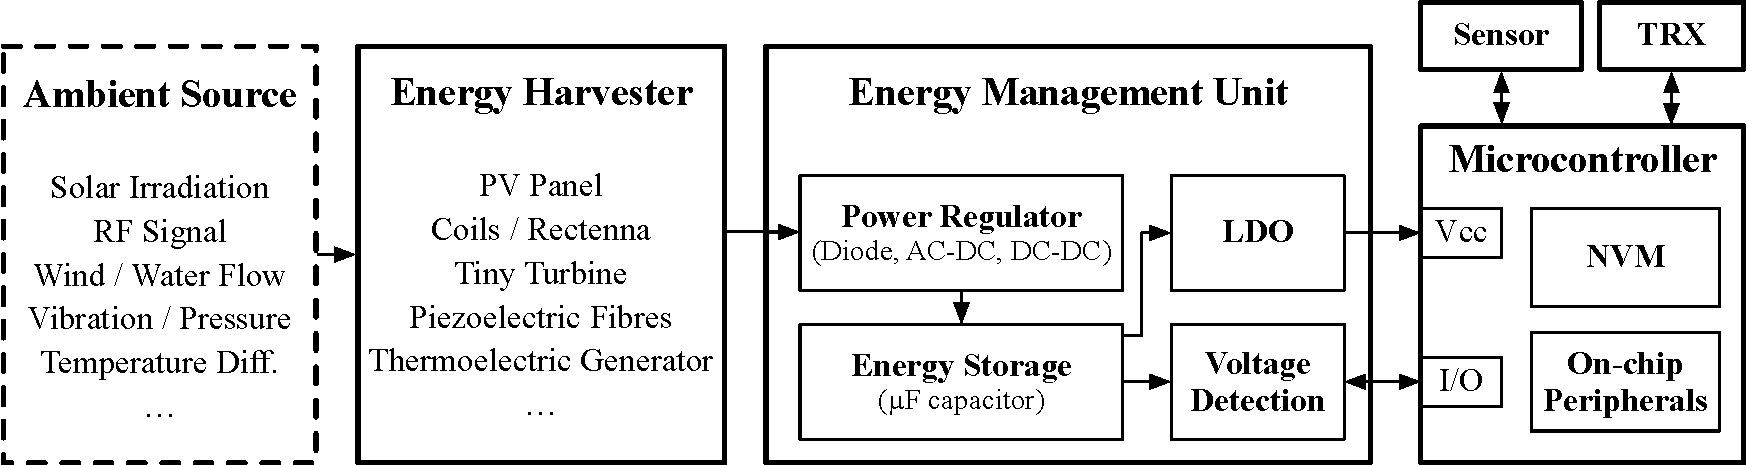
\includegraphics[width=\columnwidth]{ch1_intro/figures/IPSarch}
  \caption{A conceptual architecture of an IPS.}
  \label{fig:ips_arch}
\end{figure}

\todo[inline]{A bit unnecessary to show the details of Harvester and Source in Figure 1.}

A conceptual architecture of an typical energy-harvesting IPS is shown in \fref{fig:ips_arch}.
The power frontend is an energy harvester, which transduces an ambient energy source into electric power. 
Then, a power regulator converts the harvested power to a suitable voltage that charges up the energy storage.
The type of the power regulator depends on the pattern of the power input, which can be an AC-DC converter for AC input (e.g. a rectenna), or a DC-DC converter or a diode for DC input (e.g. a PV panel). 
The energy storage is in the form of a \SI{}{\micro\farad}-level capacitor, which buffers a small amount of energy for the load to operate intermittently in short active cycles.
The power given to the load is usually conditioned through a low-dropout regulator (LDO) to lower down supply voltage, and hence current consumption. 
IPSs are usually equipped with a voltage detection circuit so as to wake up or power up the load when the voltage of the energy storage reaches a threshold. 
In IPSs, the load is typically a microcontroller (MCU) with NVM to sustain computing state, and with many on-chip or external peripherals, e.g. sensors and wireless transceivers (TRX). 

%%% Further explanation on proactive and reactive IPSs

% Proactive approaches can be further divided into \textit{checkpointing} and \textit{task-based} ones. 
% The checkpointing approaches save and restore the whole volatile state at programmer-inserted \textit{checkpoints} (in the form of a function call), whereas task-based approaches transfer modified data at \textit{task boundaries} and are technically implemented as compiler support and programming models. 
% Once the program passes a checkpoint or task boundary, a certain amount of forward progress is achieved; otherwise, if interrupted by a power failure, the program rolls back to the last checkpoint or task boundary. 
% Both checkpoints and tasks boundaries should be carefully placed to meet atomicity and idempotency, and avoid non-termination due to energy depletion. 

% Reactive approaches can also be further divided into 



%%% Old writing

% Recently, there are two research topics in storage-less energy harvesting computing: intermittent computing (IC) and power-neutral (PN) computing. 
% A summary of this research trend in energy harvesting computing is shown in~\fref{Figure:paradigm}. 
% Briefly speaking, intermittent computing maintains system computing state after power outages, and PN computing aims to make more progress from available power by matching system power consumption with power harvested instantaneously.
% \begin{figure}[!htb]
%   \centering
%   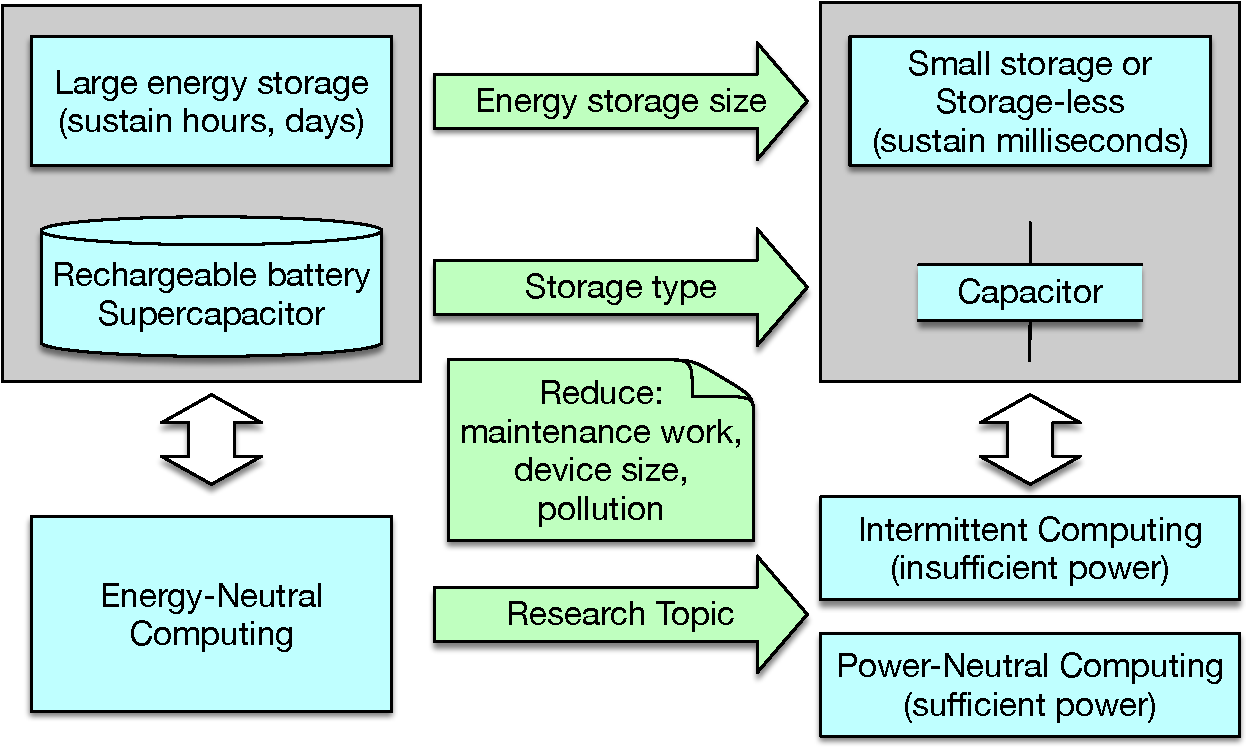
\includegraphics[width=0.7\columnwidth]{figure/intro/paradigm}
%   \caption{Research trend in energy harvesting computing: towards minimizing energy storage.}
%   \label{Figure:paradigm}
% \end{figure}

% Intermittent computing aims to maintain system volatile state after power outages with low time and energy overheads, so as to ensure forward execution and computation correctness of applications~\cite{ransford2012mementos}. Approaches in intermittent computing fundamentally diverge due to different design goals and can be classified into five categories: checkpointing, reactive, harvest-store-use, task-based, and non-volatile processors. Each of these approaches has one or a few advantages on reducing the number of system snapshots during a power cycle, reducing the size of system snapshots, minimizing hardware dependency, etc~\cite{sliper2018enabling}. 

% PN computing aims to make more progress from available power by matching system power consumption with power harvested instantaneously. PN computing dynamically adapts system performance, typically by scaling CPU clock frequency, to match the instantaneous system power consumption with the instantaneous harvested power~\cite{balsamo2016graceful, fletcher2017power}. By such performance adaptation, PN systems immediately consume excessive harvested power, prolong system active time when the harvested power drops, and reduce the frequency of system state saving and restoring operations.

\section{Applications of Energy-Harvesting IPSs}

\todo[inline]{This part intends to illustrate the key performance metric of IPSs through example applications, but it doesn't seem to directly make the point yet. }

An inherent limitation of IPSs is that the system can only execute when there is available power, as opposed to an EN system where it can still executes with buffered energy if ambient power is not available. 
This limitation thereby indicates that \textit{application operation periods and power availability should be compatible in time}. 
While there are various needs of operation periods for various application scenarios, the power availability is constrained and determined by the availability of the target energy source in the deployed environment. 
Hence, the applications of IPSs should suit, or be adapted to suit, the power availability. 
Under this consideration, there are two typical categories of application scenarios as seen in recent publications. 

To summarise the application suitability of IPSs, a diagram is shown in~\fref{fig:appsuit}. 
An example unsuitable application can be a periodic sensing task without periodically available power or the period of the energy source does not match the sensing period (left bottom circle in~\fref{fig:appsuit}).

\begin{figure}
  \centering
  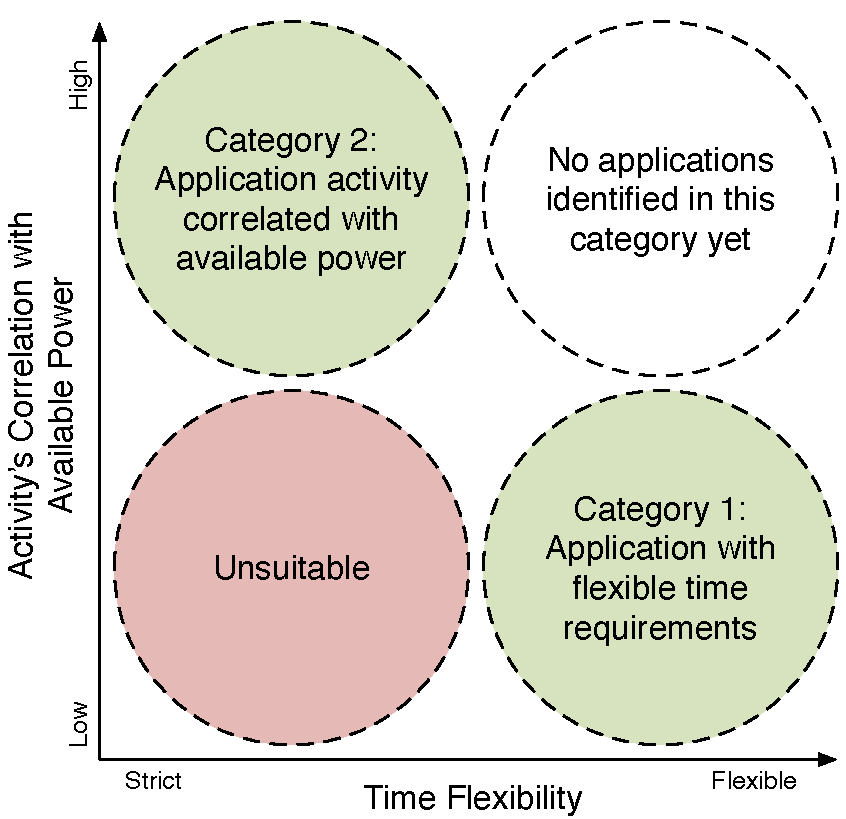
\includegraphics[width=0.7\columnwidth]{ch1_intro/figures/appsuit2}
  \caption{Application Suitability of Energy-Harvesting IPSs.}
  \label{fig:appsuit}
\end{figure}


\begin{itemize}

  \item \textbf{Category 1: Applications with flexible time requirements.}
  
  Applications with flexible requirements on operating periods tolerate the intermittency of energy sources. In such applications, devices are allowed to wait for power-on periods to execute.
  % Example energy sources could be outdoor solar energy, indoor radio-frequency (RF) energy, and human body thermal energy. Given such energy conditions, the application can process information irrelevant to the energy sources. As such energy sources are probably available in scattered and irregular periods, the application should wait for energy-available periods to activate execution. Delay-insensitive applications tolerate flexible operation periods, and hence, are suitable for such energy conditions.

  \textbf{Application 1: Kitchen event detection} 
  
  This application intends to capture kitchen events, such as dishwasher working, fan on, and refrigerator cooling, to record equipment usage. 
  As such events usually last for tens of seconds to a few hours, the device does not need to operate immediately after the event occurs or disappears. 
  An implementation of this application is shown by Maeng \textit{et al.}~\cite{maeng2019supporting}. 
  The device iterates the following tasks in turn during power-on periods: sampling acoustic information from a microphone, classifying kitchen events with a pre-trained model, and transmitting the results in Bluetooth Low-Energy (BLE) packets to an always-on server. 
  The device harvests RF energy from a dedicated RFID reader, and the packets are transmitted every a few seconds as reported. 
  This application is to complete program iterations as frequently as possible so as to improve the accuracy of event records. 

  \textbf{Application 2: Temperature monitor for air conditioning}

  This application intends to monitor indoor temperature for air conditioning. 
  As the room temperature does not usually change over a few minutes, the temperature monitor does not need to wake up frequently or periodically. 
  An implementation of this application is shown by Colin \textit{et al.}~\cite{colin2018reconfigurable}. 
  During power-on periods, the device samples temperature by an external analog sensor. 
  If the temperature is detected to be out of a pre-defined range, the device sends a BLE packet to alarm the server. 
  The device is also powered by a dedicated RFID reader. 
  Similar to Application 1, the device is expected to maximise sampling frequency in order to capture out-of-range temperature as soon as possible.

  \item \textbf{Category 2: Application activity in correlation with available power.}
  
  In such applications, the required operation periods correlate with power-on periods. 
  This correlation is typically linked by an event that comes with harvestable power. 
  When the event occurs, the device is activated by harvesting the power of the event at the same time to start operating. 
  Therefore, the application operation periods and the power availability are inherently simultaneous in such applications. 

  \textbf{Application 3: Bicycle trip counter}

  The bicycle trip counter intends to read cycling speeds and calculate total travelled distances. 
  The wheel rotation brings energy for the device to sense the cycling speed; the device does not need to operate without cycle movement. 
  The trip counter is designed as a nail-sized board installed on the frame of a bicycle, with a magnet on the wheel that brings electromagnetic energy to the system~\cite{bing2018energy}. 
  Every round of wheel rotation activates the trip counter to calculate the current speed and log the traveled distance. 
  After collecting enough energy over a few cycling rounds, the trip counter transmits the logged information. 
  This application is also expected to report results as frequently as possible. 

  \textbf{Application 4: Power meter}

  The power meter measures the power flow of a main load wire. 
  The AC power in the wire can be harvested by a coil to activate the power meter. 
  A design is shown in Monjolo~\cite{debruin2013monjolo}, where the power meter transmits a plain packet to a server once it collects a preset amount of energy. 
  The server then calculates the elapsed time between the recent two packets to estimate the main load power. 

\end{itemize}
  
As shown in the above application, a common application specification of IPSs is to do as much 'work' as possible under the same energy conditions, e.g. completing program iterations as frequently as possible, because the energy cannot be saved for later use. 
Other types of 'work' could include improving sensing accuracy or processing offloaded tasks received from other devices. 
To generally describe the 'work', in IPSs, \textit{forward progress} denotes the effective application progress, excluding lost progress due to power failures and the progress on saving and restoring state~\cite{7478428}.
As indicated by the above applications, an IPS should maximise forward progress using the limited energy. 

% \subsection{General Architecture of Energy Harvesting Sensor Nodes}

% According to recent publications of energy harvesting computing~\cite{naderiparizi2015wispcam, gomez2016dynamic, sun2017maximum, wang2016storage, balsamo2016graceful, gomez2017wearable, buchli2014dynamic}, a typical architecture of energy harvesting sensor nodes is shown in~\fref{Figure:architecture}. There are five major components: energy harvester, power management unit (PMU), energy storage, voltage converter, and load. 

% \begin{figure}[!htb]
%   \centering
%   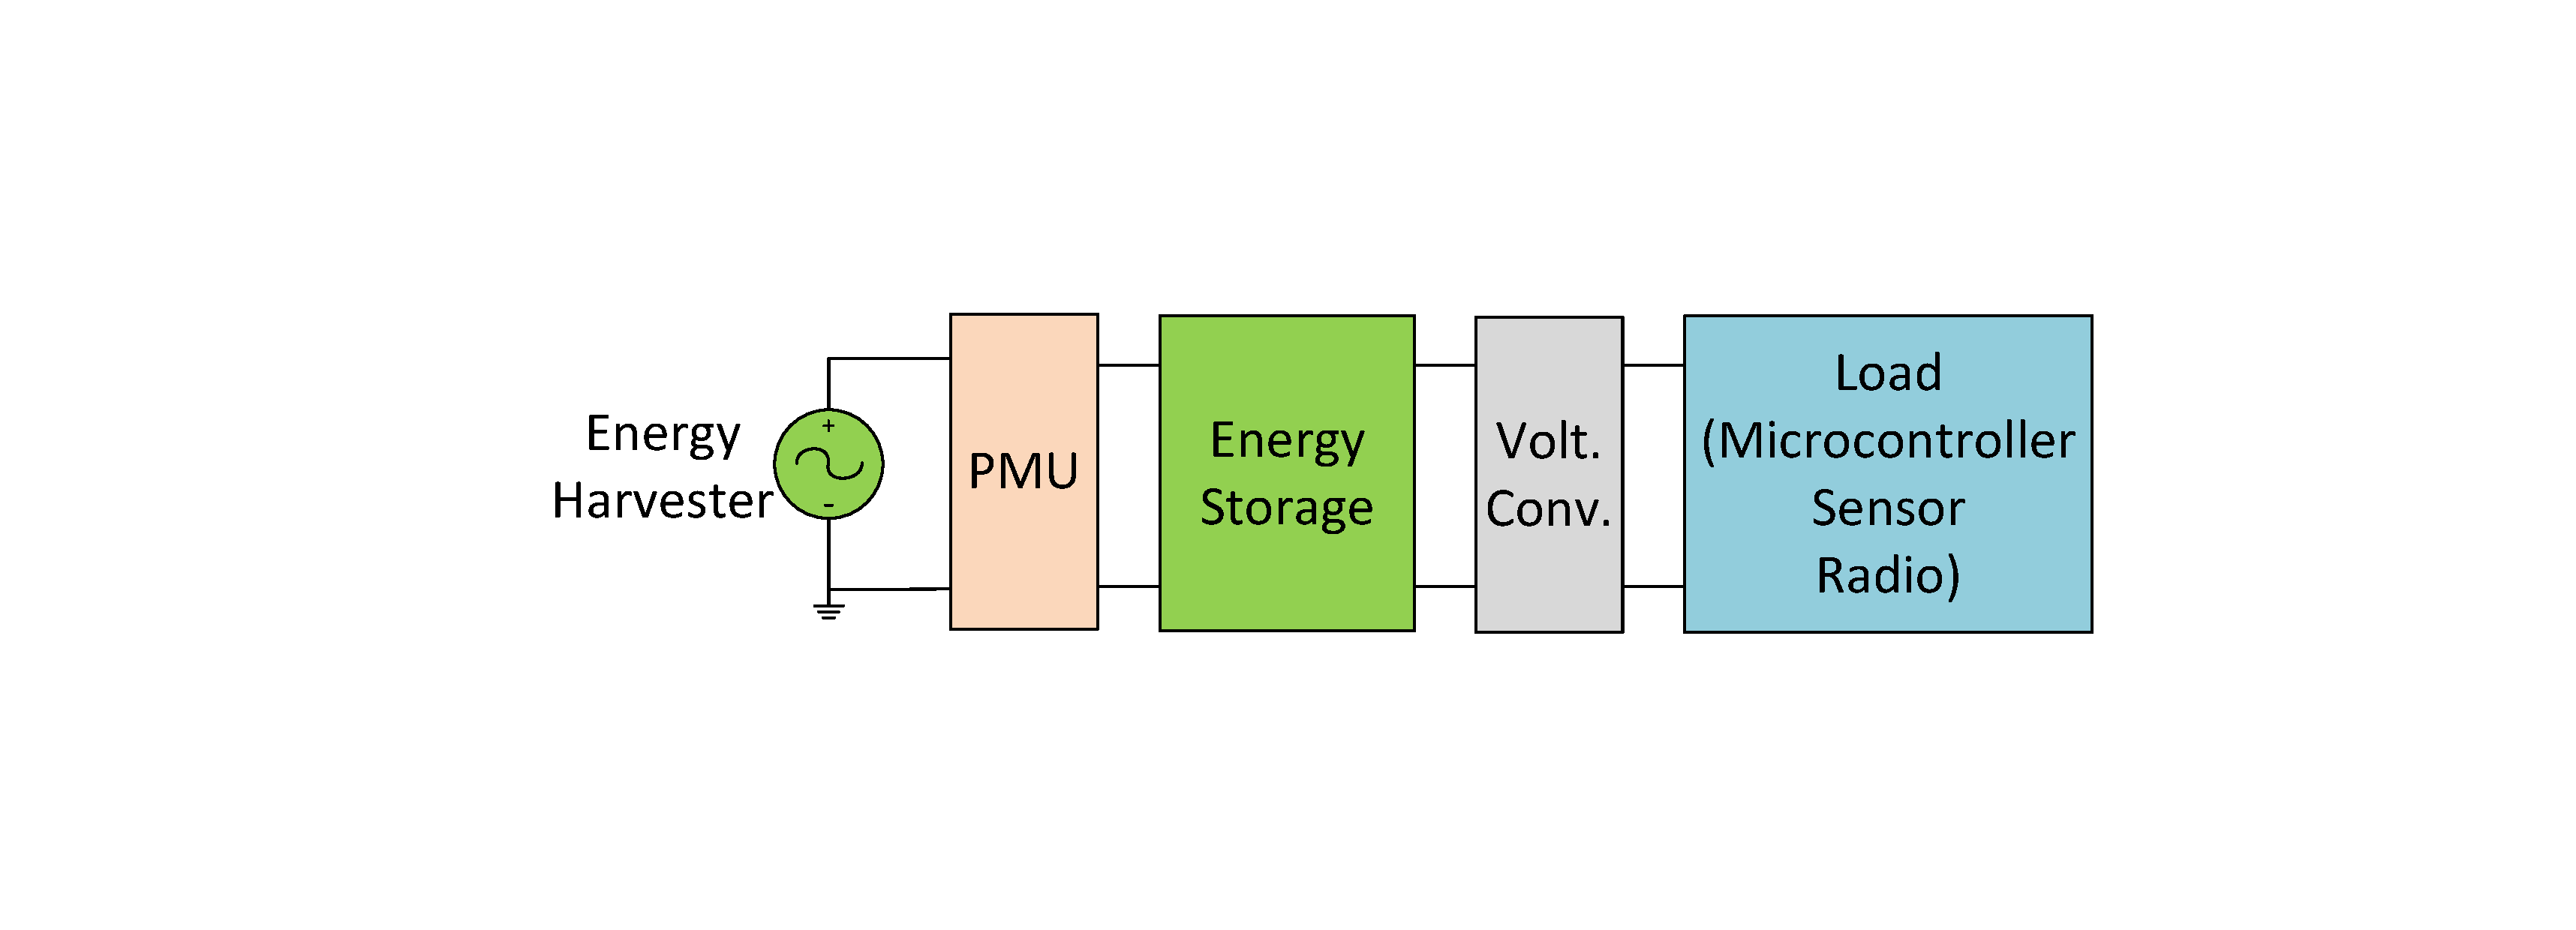
\includegraphics[width=13cm]{figure/intro/architecture}
%   \caption{Typical architecture of energy harvesting sensor nodes.}
%   \label{Figure:architecture}
% \end{figure}

% The energy harvester is the only power source in such nodes. The harvested power is then transferred to the energy storage, in some cases through a PMU. The function of PMU is to efficiently convert harvested voltage and current to an operational state for the energy storage and the load, e.g. to maximize the harvested power from the energy harvester by controlling operating voltage in systems powered by photovoltaic (PV) panels~\cite{wang2016storage, sun2017maximum, patel2008maximum}. The energy storage acts as a buffer to smooth out the inevitable and frequent temporal disparity between power harvested and power consumed, which is designed as either a rechargeable battery with a large capacity and a short lifetime, or a supercapacitor with a small capacity and a long lifetime, or in a hybrid form~\cite{xie2013charge}. With recent advances in IC, this energy storage can be minimized to a decoupling capacitor or even eliminated (no additional storage). The energy in the storage is then consumed by the load. Usually, when the terminal voltage of the energy storage does not match the operating voltage of the load, voltage conversion circuits (such as a voltage regulator, a DC-DC converter, or a low-dropout regulator) are required to provide a voltage output within the load operating range~\cite{naderiparizi2015wispcam, gomez2016dynamic, wu2012efficient}. The load, in a typical IoT application, is normally a microcontroller (MCU) with one or a few sensors and a radio. 

\section{Research Justification}

% Self-powered devices solely rely on energy harvesters to power themselves. 
% Energy harvesting power supply varies over time due to uncontrollable environmental conditions. 
% Due to the lifespan, pollution, dimension problems of batteries and supercapacitors, there is a demand for adapting computing architecture to energy harvesting supply with small storage, e.g. a capacitor. 
% Various approaches in intermittent computing and PN computing emerge to enable and improve energy harvesting computing in the scenario of minimized storage in order to reduce dimensions and cost as well as to increase lifespan of IoT devices. 

As illustrated with the previous background and application examples, a major target for many IPS approaches is to maximise forward progress given restricted energy condition. 
Various approaches have been proposed for the load to efficiently sustain computing state across power failures, so as to leave more energy for forward progress. 
However, energy efficiency can not only be explored from the load side, but can also be explored from a system perspective, where the energy allocation of IPSs has not yet been widely studied. 
The energy allocation of IPSs are mainly represented in two specifications -- the system energy storage size and the voltage threshold to wake up the load. 
Together, they determine the energy budget of one power-on cycle (but they do not change the energy input). 
This thesis will focus on how to improve the energy allocation of IPSs in order to increase forward progress, where it can be further discussed on three issues. 

% 1
% However, a larger storage than the minimum one can reduce the frequency of power outages and increase flexibility in power management, which may benefit the application throughput. 
% % 2
% Hence, there is a trade-off in sizing energy storage. 
% Apart from energy storage, the size of energy harvesters should also be considered based on a set of factors, such as system power consumption, performance requirements, energy utilization, device dimensions, and cost. 

\begin{enumerate}

\item 
% A variety of methods in intermittent computing have been proposed to overcome power outages during execution, ensuring forward execution~\cite{ransford2012mementos}, memory consistency~\cite{lucia2015simpler}, peripheral re-configuration~\cite{liu2019130}, etc. 
% Such approaches usually adopt only a minimum amount of energy storage which only allow systems to complete state saving and restoring operations before and after power outages. 
% This effect is especially noticeable in reactive intermittent systems (\sref{Section:reactiveic}), where the energy and time overheads of saving and restoring operations are proportional to the frequency of power outages. 
% On the other hand, increasing energy storage also increases the system leakage power and affects the reactivity (the energy and the charging time to activate devices) of IPSs~\cite{colin2018reconfigurable, wu2018extensible}. 
% The trade-off of scaling energy storage in intermittent computing systems should be fully studied.
With the goal of minimising device dimensions and interruption periods, most IPS approaches adopt a minimum amount of energy storage~\cite{balsamo2016hibernus++, 10.1145/2700249, 10.1145/2809695.2809707, 10.1145/3281300, 222579}. 
This is typically just sufficient for the most energy-expensive atomic operation, e.g. saving and restoring a complete state~\cite{balsamo2015hibernus}. 
However, a system with minimum energy storage may frequently go through a cycle of: wake up, restore state, execute program, save state, and halt. 
Provisioning more energy storage can prolong the power-on cycles, reduce the overheads, and hence increase forward progress, but can also increase system leakage and decrease forward progress. 
The sizing effect of energy storage on forward progress has not been studied. 
Therefore, a focus of this thesis will be studying the relationship between energy storage capacitance and forward progress in IPSs. 

\item 
% The size of energy harvesters significantly determines the amount of harvested power. 
% Undersized energy harvesters constrain available power, affecting the maximum performance of devices; oversized energy harvesters provides redundant energy, which cannot be consumed on useful work and is wasted in circuitry or never harvested, affecting the utilization of energy harvesters and unnecessarily increasing device costs. 
% Besides, the size of energy harvesters contributes to a large part in device dimensions, which may violate the size constraint of autonomous devices~\cite{buchli2014dynamic}. 
Extending the above sizing effect, to determine a size of energy storage of IPSs in deployment, developers may consider, along with forward progress, other design factors, e.g. devices' physical volume and interruption periods. 
An approach for exploring the sizing effect of energy storage on multiple design factors has not been proposed yet. 
Also, there is not a method of determining an energy storage size that balances different design factors. 
Hence, another focus of this thesis will be exploring an energy storage sizing approach for IPSs that balances multiple design factors in deployment.  

\item 
Apart from the energy storage size, the voltage threshold that wakes up an IPS also determines the energy budget of one power-on cycle. 
Existing approaches use one or a few fixed voltage thresholds, which are calibrated at design time. 
Some approaches (e.g.~\cite{gomez2016dynamic}) minimise the threshold for each task, but the fixed threshold can be violated at runtime due to variability in energy consumption, leaving the system in non-termination. 
The variable energy consumption can come from many reasons, which include, but not limited to, variability in data amounts, peripheral configurations, devices, and capacitance degradation. 
In contrast, some approaches (e.g.~\cite{maeng2019supporting}) set a universal high threshold, such that the energy budget should be mostly enough for all tasks. 
However, waiting for a high voltage threshold can be energy-inefficient because, typically, current input reduces with higher voltage and a high operating voltage also increases system quiescent current consumption. 
Hence, the final focus of this thesis will be the scheme of voltage threshold settings that avoids non-termination under runtime variable energy consumption while maintains system energy efficiency. 

\end{enumerate}

\section{Research Questions}

Motivated by the previous discussion, the following three research questions are derived:

% Questions
% 1. Does sizing the energy storage capacity has an effect on the performance of IPSs? If so, why and how? 
% 2. How can developers decide the size of energy storage? (This question may be challenged by “what about other energy storage architecture?”)
% 3. After addressing the efficiency of computing tasks, how can the devices perform atomic tasks, e.g. peripheral operations. (After this question, my previous questions may be challenged by “why doesn’t that encompass atomic tasks?”)

% \item[1.] What is the effect of energy storage capacity and energy harvester size on the behaviours of intermittent computing systems?

% Adding energy storage to intermittent computing systems may reduce state saving and restoring overheads and tolerate larger atomic operations, but may also increase leakage power, device dimensions, and undermine system reactivity. Energy harvester sizing also affects multiple outcomes, such as system performance requirement, device dimensions, and costs. System behaviours include application throughput, active time, reactivity, frequency and overheads of state saving and restoring operations, and energy utilization. 

% \item[2.] How can designers size energy harvesters and energy storage in IC systems to maximize application throughput while meeting requirements for device dimensions and costs?

% Based on the analysis of sizing effect on system behaviours, this question focuses on practical concerns when deploying IoT sensor nodes. A sizing tool should be provided, where the user should import the energy source conditions at the deploying location. This tool should provide a spectrum of energy harvester and storage sizes with corresponding outcomes of each sizing choice.

\begin{enumerate}

\item What is the effect of sizing the energy storage capacity on the performance of IPSs? 

Specifically, the energy storage capacity in IPSs is presented as the capacitance between \nm{V}{cc} and ground. 
The forward progressing rate directly determines application performance, e.g. program iteration rate or task completion time, and hence is regarded as the performance metric in this study. 
The goal is to explore whether sizing the energy storage capacity can change the forward progressing rate in IPSs, and if so, to study and quantify the relationship between them. 

\item How may the energy storage of IPSs be sized to trade off forward progress against device dimensions and interruption periods?

While the last question explores the energy storage sizing effect on computational performance, this question encompasses more design factors in IPSs that a capacitor size can affect. 
Increasing energy storage capacity may benefit forward progress, but may also exhibit side effects. 
A larger capacitor typically has larger physical dimensions, which are a key design factor that IPSs should minimise in some application scenarios, e.g. wearable and implantable sensors. 
Also, a larger capacitor also leads to longer charge-discharge cycles, and thus prolongs interruption periods and undermines system reactivity to external events. 
The goal is to study the trade-off and to propose an approach that recommends an energy storage size for practical deployment.
% Most IPSs minimize energy storage capacity so as to minimize device dimensions and interruption periods~\cite{7442814, 10.1145/2700249, 10.1145/2809695.2809707, 10.1145/3281300, 222579}. 
% A simulation tool of IPSs should be provided, where users can define energy source conditions and energy harvester sizes. 
% The tool should be able to output the physical size of energy storage and interruption periods in certain metrics. 
% An appropriate size of energy storage can be suggested by this tool with a cost function to trade off multiple factors. 

\item How can an IPS run safely and efficiently with runtime variable energy consumption of tasks?

Energy consumption of tasks can change at runtime with regards to many factors, where we consider, but not limited to, the variability in data amounts to process, peripheral configurations, devices, and capacitor degradation. 
A design concept is to allocate just enough energy for each task.
This design concept can further break into two aspects -- safety and efficiency. 
The safety aspect means that the IPS should intend to avoid non-termination by allocating enough energy for tasks.
The efficiency aspect means that, while meeting the safety aim, the IPS should minimise the energy budget, such that the system can wait for the least possible energy threshold, maintaining energy efficiency and forward progress. 
The goal is to devise an approach that can enable IPSs to run with variable energy consumption of tasks, following the above design concept. 

% Energy profiling of tasks is done at design time in SoA approaches. 
% Energy profiling is typically necessary for tasks that are intended to complete within one active cycle, i.e. they are not supposed to be interrupted by a checkpoint or stop due to energy depletion. 
% The consumption of a task can vary at runtime due to the variability in data amounts to process, peripheral configurations, devices, and capacitor degradation. 
% It becomes necessary for IPSs to have runtime energy profiling functionality so as to overcome the impractical efforts of design-time profiling and adapt to tasks' latest energy consumption.

% \item How can an IPS efficiently and safely adapts its voltage threshold to minimize non-termination while maintain high energy efficiency? 

% Atomic operations in IPSs denote operations that should be completed in one continuous period. 
% If an atomic operation is interrupted by a power failure, it should be re-executed rather than resumed. 
% Current approaches handle atomic operations by accumulating energy to a predefined voltage threshold; after reaching that threshold, the system starts execution and re-executes the atomic section if the power fails. 
% Fixed low thresholds can be violated when any runtime variability increases energy consumption, leading to non-termination. 
% On the other hand, a universal high voltage threshold, though probably avoids non-termination, can result in long charging time, slowing down the system execution or even leaving the system in an infinite wait at low input power.
% The goal is to discover an adaptive threshold adaptation scheme that allocates an just-enough energy budget that avoids non-termination and maintain high system energy efficiency. 

% However, this threshold is typically set high enough for all atomic operations in a program, so the systems usually wait for a long charging period which wastes energy and impedes response time. 
% Also, when capacitor degrades, the predefined threshold may not provide enough energy for the same operations, so that the system cannot make forward progress. 
% A new method of utilizing energy storage to solve these two problems is necessary. 
  
\end{enumerate}

\section{Research Contributions}

\todo[inline]{Need more explanation}

% \footnote{With the limits on portability of different IC approaches, Question 1 and 2 are studied based on reactive IC methodology}

The contributions done to the address the research questions in this thesis are:
\begin{itemize}
  \item[1.] Exploration and analysis of the energy storage sizing effect on reactive intermittent computing system, where we quantify and explain the relationship between energy storage capacity and forward progress.
  \item[2.] A method and a simulation tool for sizing energy storage in deploying IPSs, where forward progress, dimensions, and interruption periods are traded off in a cost function.
  \item[3.] A runtime energy profiling and voltage threshold adaptation approach for efficiently performing atomic operations in cases of variable runtime energy consumption. 
  % \item[4.] A configurable model of reactive IC systems, including the interrelationship among energy harvesting supply, energy storage, and a processing load.
\end{itemize}


\section{Publications}

The research presented in this thesis were published in the following papers:

\begin{itemize}
    \item J. Zhan, G. V. Merrett, and A. S. Weddell. "Exploring the Effect of Energy Storage Sizing on Intermittent Computing System Performance." \textit{IEEE Transactions on Computer-Aided Design of Integrated Circuits and Systems}, 2021.~\cite{zhan2021exploring}

    \item J. Zhan, A. S. Weddell, and G. V. Merrett. "Adaptive Energy Budgeting for Atomic Operations in Intermittently-Powered Systems." In \textit{Proceedings of the 8th International Workshop on Energy Harvesting and Energy-Neutral Sensing Systems (ENSsys '20)}, pp.82-83, 2020.~\cite{zhan2020adaptive}
\end{itemize}


\section{Thesis Structure}

The remaining part of this thesis is organised as follows. 
\cref{chapter:review} provides background on energy harvesting, energy storage and energy-neutral computing, as well as reviews recent IPS techniques following a taxonomy based on their fundamental mechanisms and focusses.
\cref{chapter:sizingeffect} analyses the sizing effect of energy storage on IPS performance.
Extending \cref{chapter:sizingeffect}, \cref{chapter:sizingapproach} explores a wider energy storage sizing effect on IPSs considering multiple design factors and real-world energy conditions. 
Apart from sizing energy storage, \cref{chapter:opta} focusses on runtime energy profiling and adaptation through adaptive voltage thresholding, so as to maintain system performance despite runtime variability.
Chapter~\ref{chapter:conclusion} concludes this thesis and discusses potential directions of future research. 